\section{Controller}
The controller in this application has to be a \textbf{signal generator} that can produce a waveform that can be amplified and sent to the coil.
The controller we used for testing is an ESP32 microcontroller.
We chose this controller as the first test hardware for its \textbf{simplicity of programming} and its \textbf{integrated DAC}.

% -- Subsection 4.1
\subsection{ESP32 DAC Characteristics}
The DAC included in the ESP32 is a pretty basic one but as a first test, it is enough.
The DAC has a resolution of \textbf{8 bits}, and it can output a voltage between \textbf{0} and \textbf{3.3V} with a maximum current output of \textbf{12mA}.

\subsection{ESP32 waveform generator}
Using a simple program the ESP32 can be used as a pretty capable waveform generator.
The software we used is the \textbf{ESP32 Signal Generator} from \textbf{\href{https://corz.org}{corz.org}} \cite{corz_signal_gen}.
This software allows the user to generate the following waveforms:
\begin{itemize}
    \item Sine wave from 16Hz to 500kHz
    \item Square wave from 1Hz to 40MHz
    \item Triangle wave from 153Hz to 150kHz 
    \item Sawtooth wave from 153Hz to 150kHz
\end{itemize}

\begin{samepage}
    Between these ranges of frequencies, the generated waveforms are pretty accurate.
    \nopagebreak

    \begin{figure}[H]
        \centering
        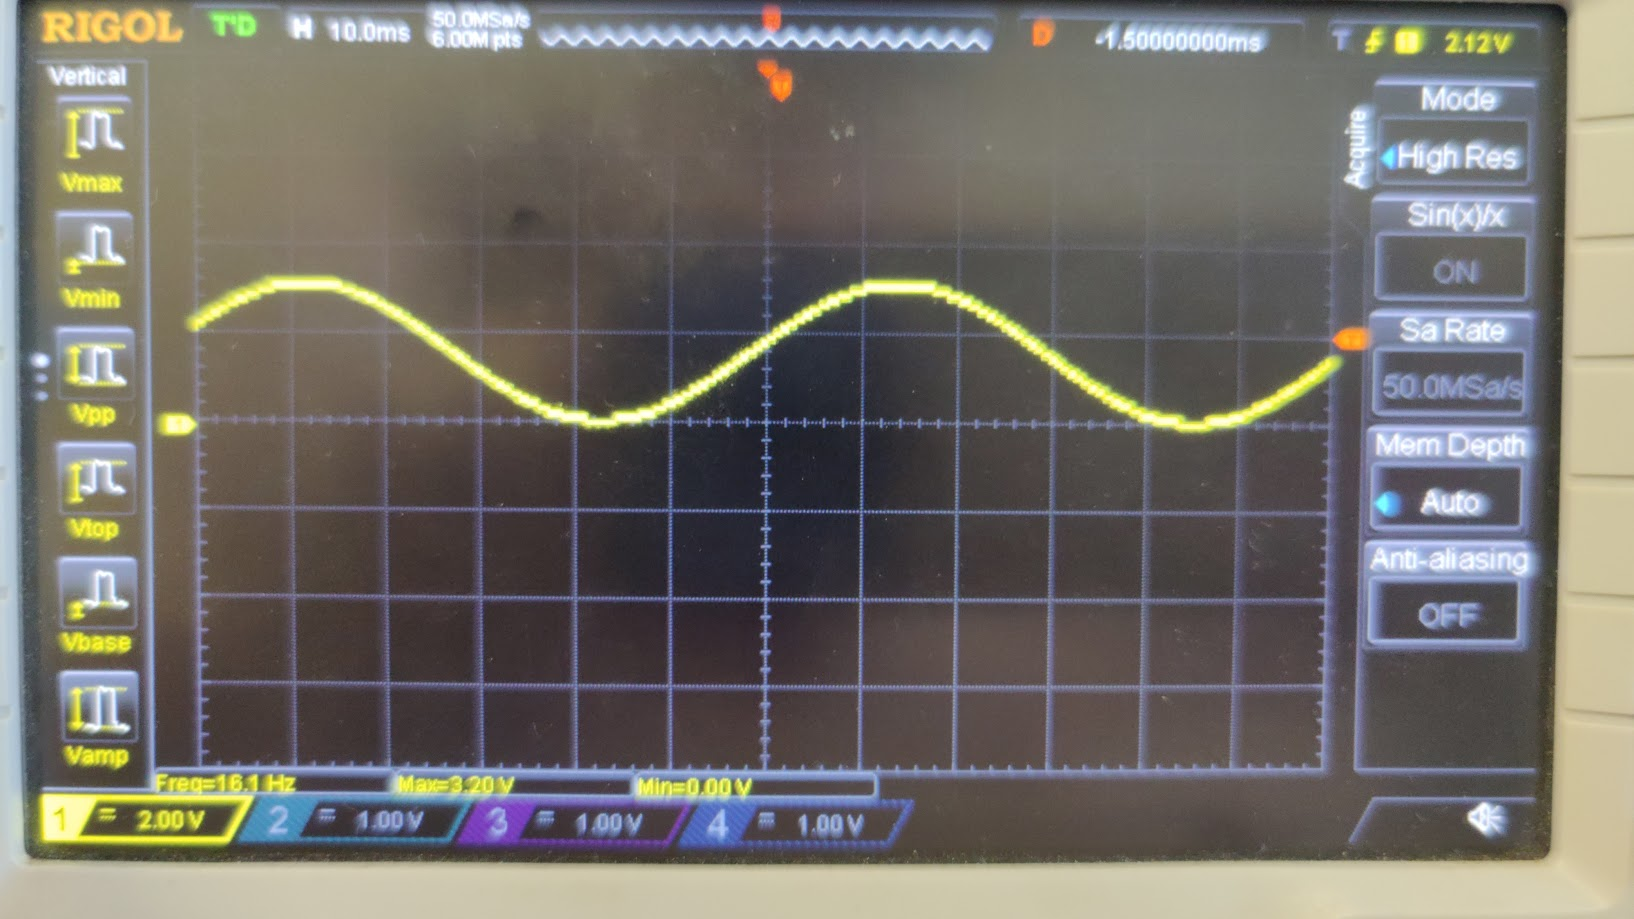
\includegraphics[width=0.9\linewidth]{Chapters/Chapter4/Figures/16Hz_signal_gen.jpg}
        \caption[ESP32 DAC in action]{ESP32 16Hz Sine wave generated by the ESP32 Signal Generator software.}
        \label{fig:16Hz_signal_gen}
    \end{figure}
\end{samepage}

\pagebreak

% \subsubsection{Esp32 DAC limitations}

% \subsubsection{Esp32 DAC Noise}
